% 2026 MRS Fall Meeting poster. Built on D. Sariturk's MaterialsFramework poster
% template (mf_poster_style.sty; header, boxes, impact numbers, TikZ vocabulary).
%
% Size: 42 x 42 in (106.68 x 106.68 cm). Same content as ../poster_2026_MRS_fall (46 x 42 in).
%   MRS Fall 2026 poster space: 46 x 46 in, two posters per board.
%   TAMU Zachry helpdesk plotter (HP DesignJet, ZACH 383): 42 in roll.
% Compile: tectonic poster.tex   (or xelatex / lualatex on Overleaf)
\documentclass[final]{beamer}
\usepackage[orientation=landscape,size=custom,width=106.68,height=106.68,scale=1.15]{beamerposter}
\usepackage{mf_poster_style}

\graphicspath{{./}}

\renewcommand{\bodyfont}{\fontsize{33}{39.8}\selectfont}
\renewcommand{\capfont}{\fontsize{27.5}{33.1}\selectfont}

% --- geometry for the 42 x 42 in page (template defaults are for 48 x 36 in)
\setlength{\headerdepth}{13.6cm}          % taller band: two-line, extra-large title
\setlength{\headerhalf}{0.5\headerdepth}
\renewcommand{\contentstart}{11.05cm}
\renewcommand{\colw}{0.26}
\renewcommand{\midcolw}{0.44}
\setlength{\colheight}{82.3cm}
\newcommand{\footeranchor}{-99.14cm}      % page height minus 7.54 cm, as in the template

\hyphenpenalty=10000
\exhyphenpenalty=10000
\tolerance=9999
\emergencystretch=3em

\newcommand{\figcaptionc}[1]{%
  \par\vspace{0.25cm}
  {\raggedright\capfont\color{DarkGrey} #1\par}%
}
\newcommand{\secno}[1]{{\color{DarkGrey}#1\enspace}}
% impact number with a caption-sized label (the template's \impactnumber uses \small)
\newcommand{\keynumber}[3][66]{%
  \begin{minipage}[t]{0.31\linewidth}
  \centering
  {\titlefont\bfseries\fontsize{#1}{#1}\selectfont\color{AggieMaroon} #2}\\[0.30cm]
  {\fontsize{25}{30}\selectfont #3\par}
  \end{minipage}%
}

% References + Acknowledgements + two QR panels.
\newcommand{\gatefooter}[2]{%
\begin{tikzpicture}[remember picture,overlay]
  \node[anchor=north west,inner sep=0pt] at
    ([xshift=\sidemargin,yshift=\footeranchor]current page.north west) {%
    \begin{minipage}[t]{\textwidth}
    \begin{columns}[T,totalwidth=\textwidth]
      \begin{column}{0.43\textwidth}
        {\headfont\bfseries\Large\color{AggieMaroon} References}\\[0.25cm]
        {\small\raggedright\color{DarkGrey} #1\par}
      \end{column}
      \begin{column}{0.33\textwidth}
        {\headfont\bfseries\Large\color{AggieMaroon} Acknowledgements}\\[0.25cm]
        {\small\raggedright\color{DarkGrey} #2\par}
      \end{column}
      \begin{column}{0.20\textwidth}
        \setqrboxw\vspace*{0.56cm}\par
        \hfill
        \begin{minipage}[t]{\qrboxw}\qrpanel{https://github.com/sheikhahnaf/matgen-BO}{Code and data}\end{minipage}%
        \hspace{0.9cm}%
        \begin{minipage}[t]{\qrboxw}\qrpanel{https://doi.org/10.57967/hf/9893}{Checkpoints}\end{minipage}%
        \hspace*{0.3cm}
      \end{column}
    \end{columns}
    \end{minipage}};
\end{tikzpicture}%
}

% Surrogate-gated loop, drawn in the visual vocabulary of the template's own
% TikZ figures (grey layer boxes, maroon flow arrows, white chips, maroon band).
\newcommand{\loopdiagram}{%
\resizebox{\linewidth}{!}{%
\begin{tikzpicture}[
  x=1cm,y=1cm,
  layer/.style = {draw=DarkGrey,line width=1.4pt,rounded corners=5pt,fill=PanelGrey},
  lbl/.style   = {font=\fontsize{28}{32}\selectfont\bfseries,text=AggieMaroon},
  sub/.style   = {font=\fontsize{22}{26}\selectfont,text=DarkGrey},
  note/.style  = {font=\fontsize{22}{26}\selectfont,text=DarkGrey},
  notem/.style = {font=\fontsize{23}{27}\selectfont\bfseries,text=AggieMaroon},
  chip/.style  = {draw=DarkGrey,line width=1.2pt,rounded corners=3pt,fill=white,
                  inner xsep=9pt,inner ysep=10pt,font=\fontsize{24}{28}\selectfont},
  flow/.style  = {-{Stealth[length=11pt,width=10pt]},AggieMaroon,line width=2.6pt},
  back/.style  = {-{Stealth[length=9pt,width=8pt]},DarkGrey,line width=1.8pt},
  bypass/.style= {-{Stealth[length=10pt,width=9pt]},DarkGrey,line width=2.2pt,
                  dash pattern=on 9pt off 6pt},
]
\def\L{2.0}      % left edge of the boxes
\def\BW{21.5}    % box width (boxes span 2.0 .. 23.5, centred on 12.75)

% ---- generator
\node[layer,minimum width=\BW cm,minimum height=6.9cm,anchor=north west]
  (gen) at (\L,30.0) {};
\node[lbl,anchor=north west] at ([shift={(0.7,-0.45)}]gen.north west) {Diffusion prior};
\node[sub,anchor=north east] at ([shift={(-0.7,-0.58)}]gen.north east)
  {MatterGen, CrystalFlow, ADiT};
\node[anchor=south,inner sep=0pt] at ([yshift=0.45cm]gen.south)
  {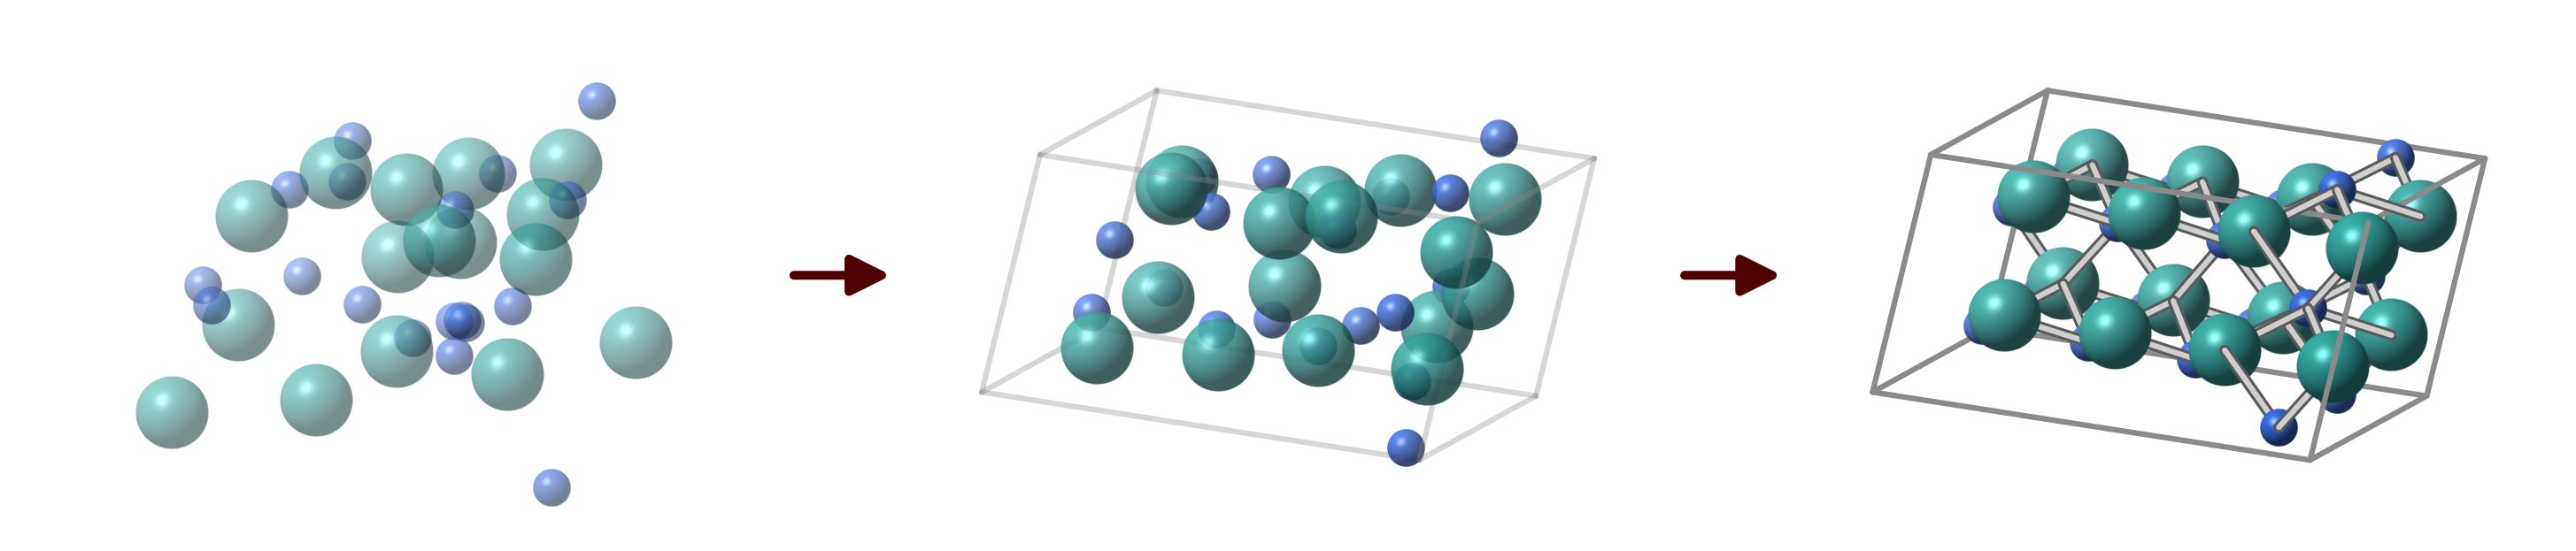
\includegraphics[width=20.6cm]{figs/fig_denoise.png}};

% ---- relax + filter
\node[layer,minimum width=\BW cm,minimum height=2.8cm,anchor=north west]
  (sun) at (\L,21.5) {};
\node[lbl,anchor=west] at ([xshift=0.7cm]sun.west) {Relax + filter};
\node[sub,anchor=east] at ([xshift=-0.7cm]sun.east) {stable, unique, novel};

% ---- the gate
\node[layer,fill=white,draw=AggieMaroon,line width=2.4pt,
      minimum width=\BW cm,minimum height=7.0cm,anchor=north west]
  (gate) at (\L,17.2) {};
\node[lbl,anchor=north west] at ([shift={(0.7,-0.45)}]gate.north west) {Gate};
\node[sub,anchor=north east] at ([shift={(-0.7,-0.58)}]gate.north east)
  {the only change to ungated fine-tuning};
\node[chip] (gp)  at ([yshift=-0.10cm]gate.center) {Gaussian process};
\node[chip,anchor=east] (orb) at ([xshift=-1.25cm]gp.west) {ORB + PCA};
\node[chip,anchor=west] (ei)  at ([xshift=1.25cm]gp.east)  {EI + diversity};
\draw[flow] (orb.east) -- (gp.west);
\draw[flow] (gp.east) -- (ei.west);
\node[note,anchor=south] at ([yshift=0.50cm]gate.south)
  {ranks every survivor; the rest earn no reward};

% ---- oracle
\node[fill=AggieMaroon,minimum width=\BW cm,minimum height=3.8cm,
      anchor=north west,rounded corners=5pt] (orc) at (\L,8.0) {};
\node[anchor=north west,text=white,font=\fontsize{28}{32}\selectfont\bfseries]
  at ([shift={(0.7,-0.50)}]orc.north west) {Property oracle};
\node[anchor=south west,text=PanelGrey,font=\fontsize{22}{26}\selectfont]
  at ([shift={(0.72,0.50)}]orc.south west)
  {learned potential: phonons ($C_p$), equation of state ($K_{\mathrm{VRH}}$)};

% ---- policy update
\node[layer,minimum width=\BW cm,minimum height=2.8cm,anchor=north west]
  (upd) at (\L,2.8) {};
\node[lbl,anchor=west] at ([xshift=0.7cm]upd.west) {Policy update};
\node[sub,anchor=east] at ([xshift=-0.7cm]upd.east) {REINFORCE};

% ---- flow
\draw[flow] (gen.south) -- (sun.north);
\node[note,anchor=west] at ([shift={(0.5,-0.80)}]gen.south) {about 16 candidates per cycle};
\draw[flow] (sun.south) -- (gate.north);
\draw[flow] ([xshift=3.4cm]gate.south) -- ([xshift=3.4cm]orc.north);
\node[notem,anchor=west] at ([shift={(3.95,-1.10)}]gate.south) {top 4 per cycle};
\draw[back] ([xshift=-3.4cm]orc.north) -- ([xshift=-3.4cm]gate.south);
\node[note,anchor=east] at ([shift={(-3.95,-1.10)}]gate.south) {labels train the GP};
\draw[flow] (orc.south) -- (upd.north);
\node[note,anchor=west] at ([shift={(0.5,-0.70)}]orc.south) {rewards};

% ---- next cycle (left) and ungated bypass (right)
\coordinate (lx) at (0.50,0);
\coordinate (rx) at (25.00,0);
\draw[flow] (upd.west) -- (lx |- upd.west) -- (lx |- gen.west) -- (gen.west);
\node[note,rotate=90,anchor=center] at (1.25,15.0) {next cycle};
\draw[bypass] (sun.east) -- (rx |- sun.east) -- (rx |- orc.east) -- (orc.east);
\node[note,rotate=-90,anchor=center] at (24.25,13.1) {ungated: every survivor is evaluated};

\end{tikzpicture}}%
}


\begin{document}
\begin{frame}[t]

\posterchrome{}{0cm}{0cm}{10}

\posterheader
  {\begin{tabular}{@{}l@{}}Surrogate-Gated Diffusion and Foundation-Model\\[0.12em]
   Embeddings for Bayesian Materials Design\end{tabular}}
  {\textbf{Sk Md Ahnaf Akif Alvi}$^{1,2}$, Jan Janssen$^{3}$, Danny Perez$^{4}$,
   Douglas Allaire$^{5}$, Raymundo Arr\'{o}yave$^{1,5,6}$}
  {$^{1}$Materials Science and Engineering, $^{5}$Mechanical Engineering, $^{6}$Industrial and Systems Engineering, Texas A\&M University\\[0.1cm]
   $^{2}$Theoretical Division and $^{4}$X Computational Physics Division, Los Alamos National Laboratory \quad
   $^{3}$Max Planck Institute for Sustainable Materials \quad ahnafalvi@tamu.edu}

\vspace*{\contentstart}

\begin{columns}[T,totalwidth=\textwidth]

%======================= COLUMN 1: problem and method =======================
\begin{postercol}{\colw\textwidth}

\begin{posterbox}{\secno{1}Motivation}
\raggedright
Diffusion models steered by reinforcement learning propose crystals
faster than any property oracle can score them, so oracle calls set the
cost of closed-loop design. Acquisition depends on how candidates are
ordered, not on their exact values. A cheap surrogate that ranks well can
therefore pick the few worth evaluating.
\end{posterbox}

\vfill

\begin{posterbox}{\secno{2}Surrogate-Gated Loop}
\centering
\loopdiagram

\vspace{0.45cm}
\raggedright
Everything else matches ungated fine-tuning (MatInvent). A 20-cycle run
makes 92 oracle calls: a 16-call warm start, then four~per~cycle.
\end{posterbox}

\vfill

\begin{posterbox}{\secno{3}Choosing the Surrogate}
\centering
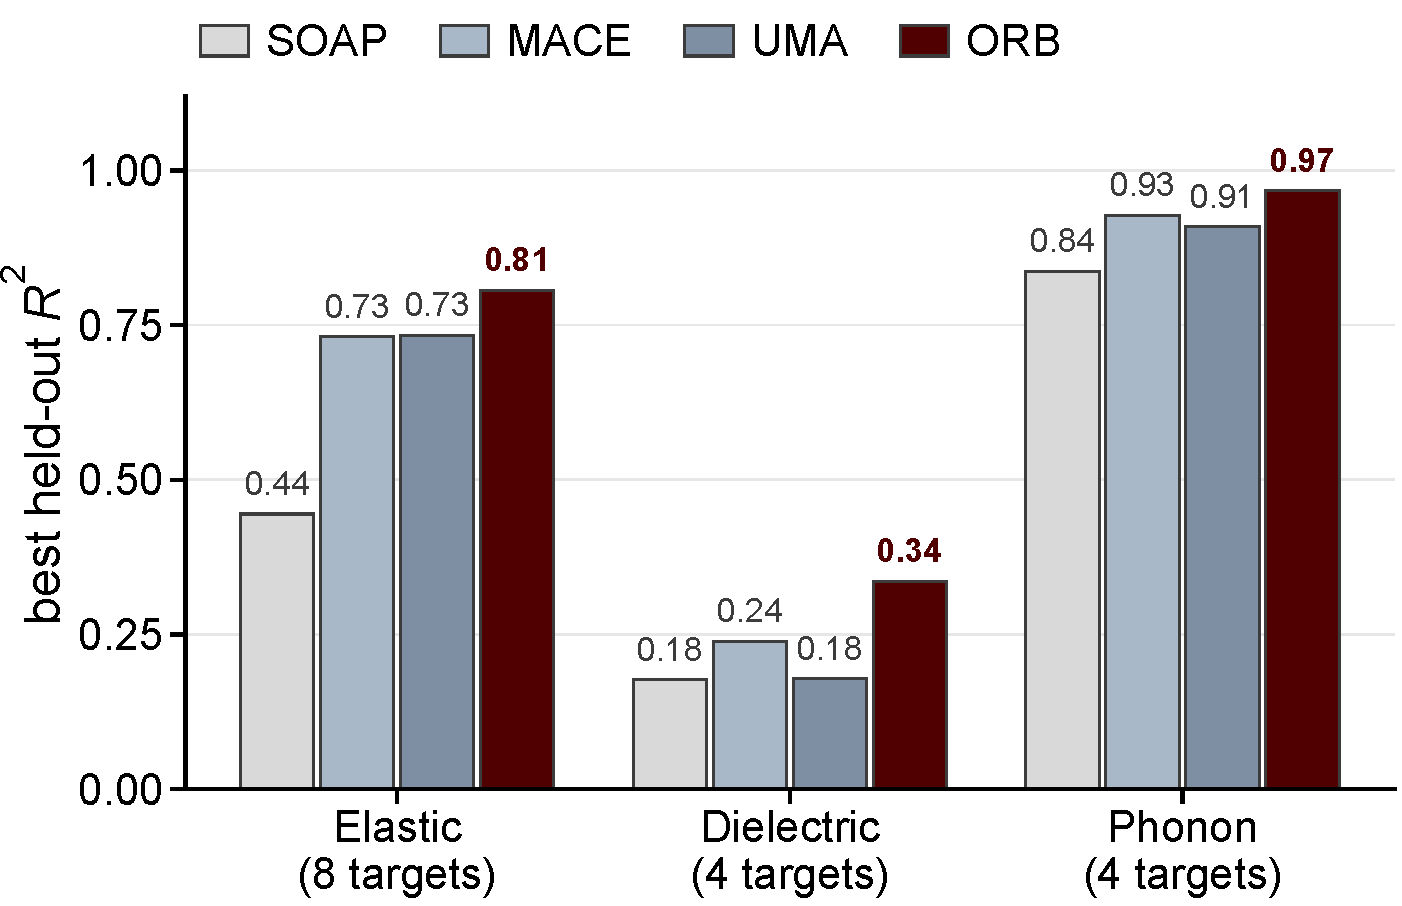
\includegraphics[width=\linewidth]{figs/fig_benchmark.pdf}

\vspace{0.30cm}
\raggedright
From 8{,}640 fits over featurizers, surrogates and training sizes,
pretrained ORB embeddings rank first on all three datasets. A Gaussian
process on 50 principal components is the stable default.
\end{posterbox}

\end{postercol}

%======================= COLUMN 2: main results =======================
\begin{postercol}{\midcolw\textwidth}

\begin{posterbox}[colframe=AggieMaroon,boxrule=2.4pt,
                  left=1.2cm,right=1.2cm,bottom=0.8cm]{Key Findings}
{\headfont\bfseries\fontsize{45}{53}\selectfont\color{AggieMaroon}\raggedright
A Gaussian-process gate in front of the oracle matches ungated
discovery with a fraction of the evaluations.\par}
\vspace{0.75cm}
\begin{center}
\keynumber[66]{2.1--7.3\texttimes}{fewer oracle calls to match\\ungated fine-tuning, in all six cases}
\hfill
\keynumber[66]{314 vs 233}{GPa at an equal budget:\\ranked against arbitrary selection}
\hfill
\keynumber[66]{$\rho$ = 0.94}{ranks 1{,}209 unseen structures;\\oracle within 2.5\% of DFT}
\end{center}
\end{posterbox}

\vfill

\begin{posterbox}[left=0.9cm,right=0.9cm]{\secno{4}Matching Discovery with Fewer Oracle Calls}
\centering
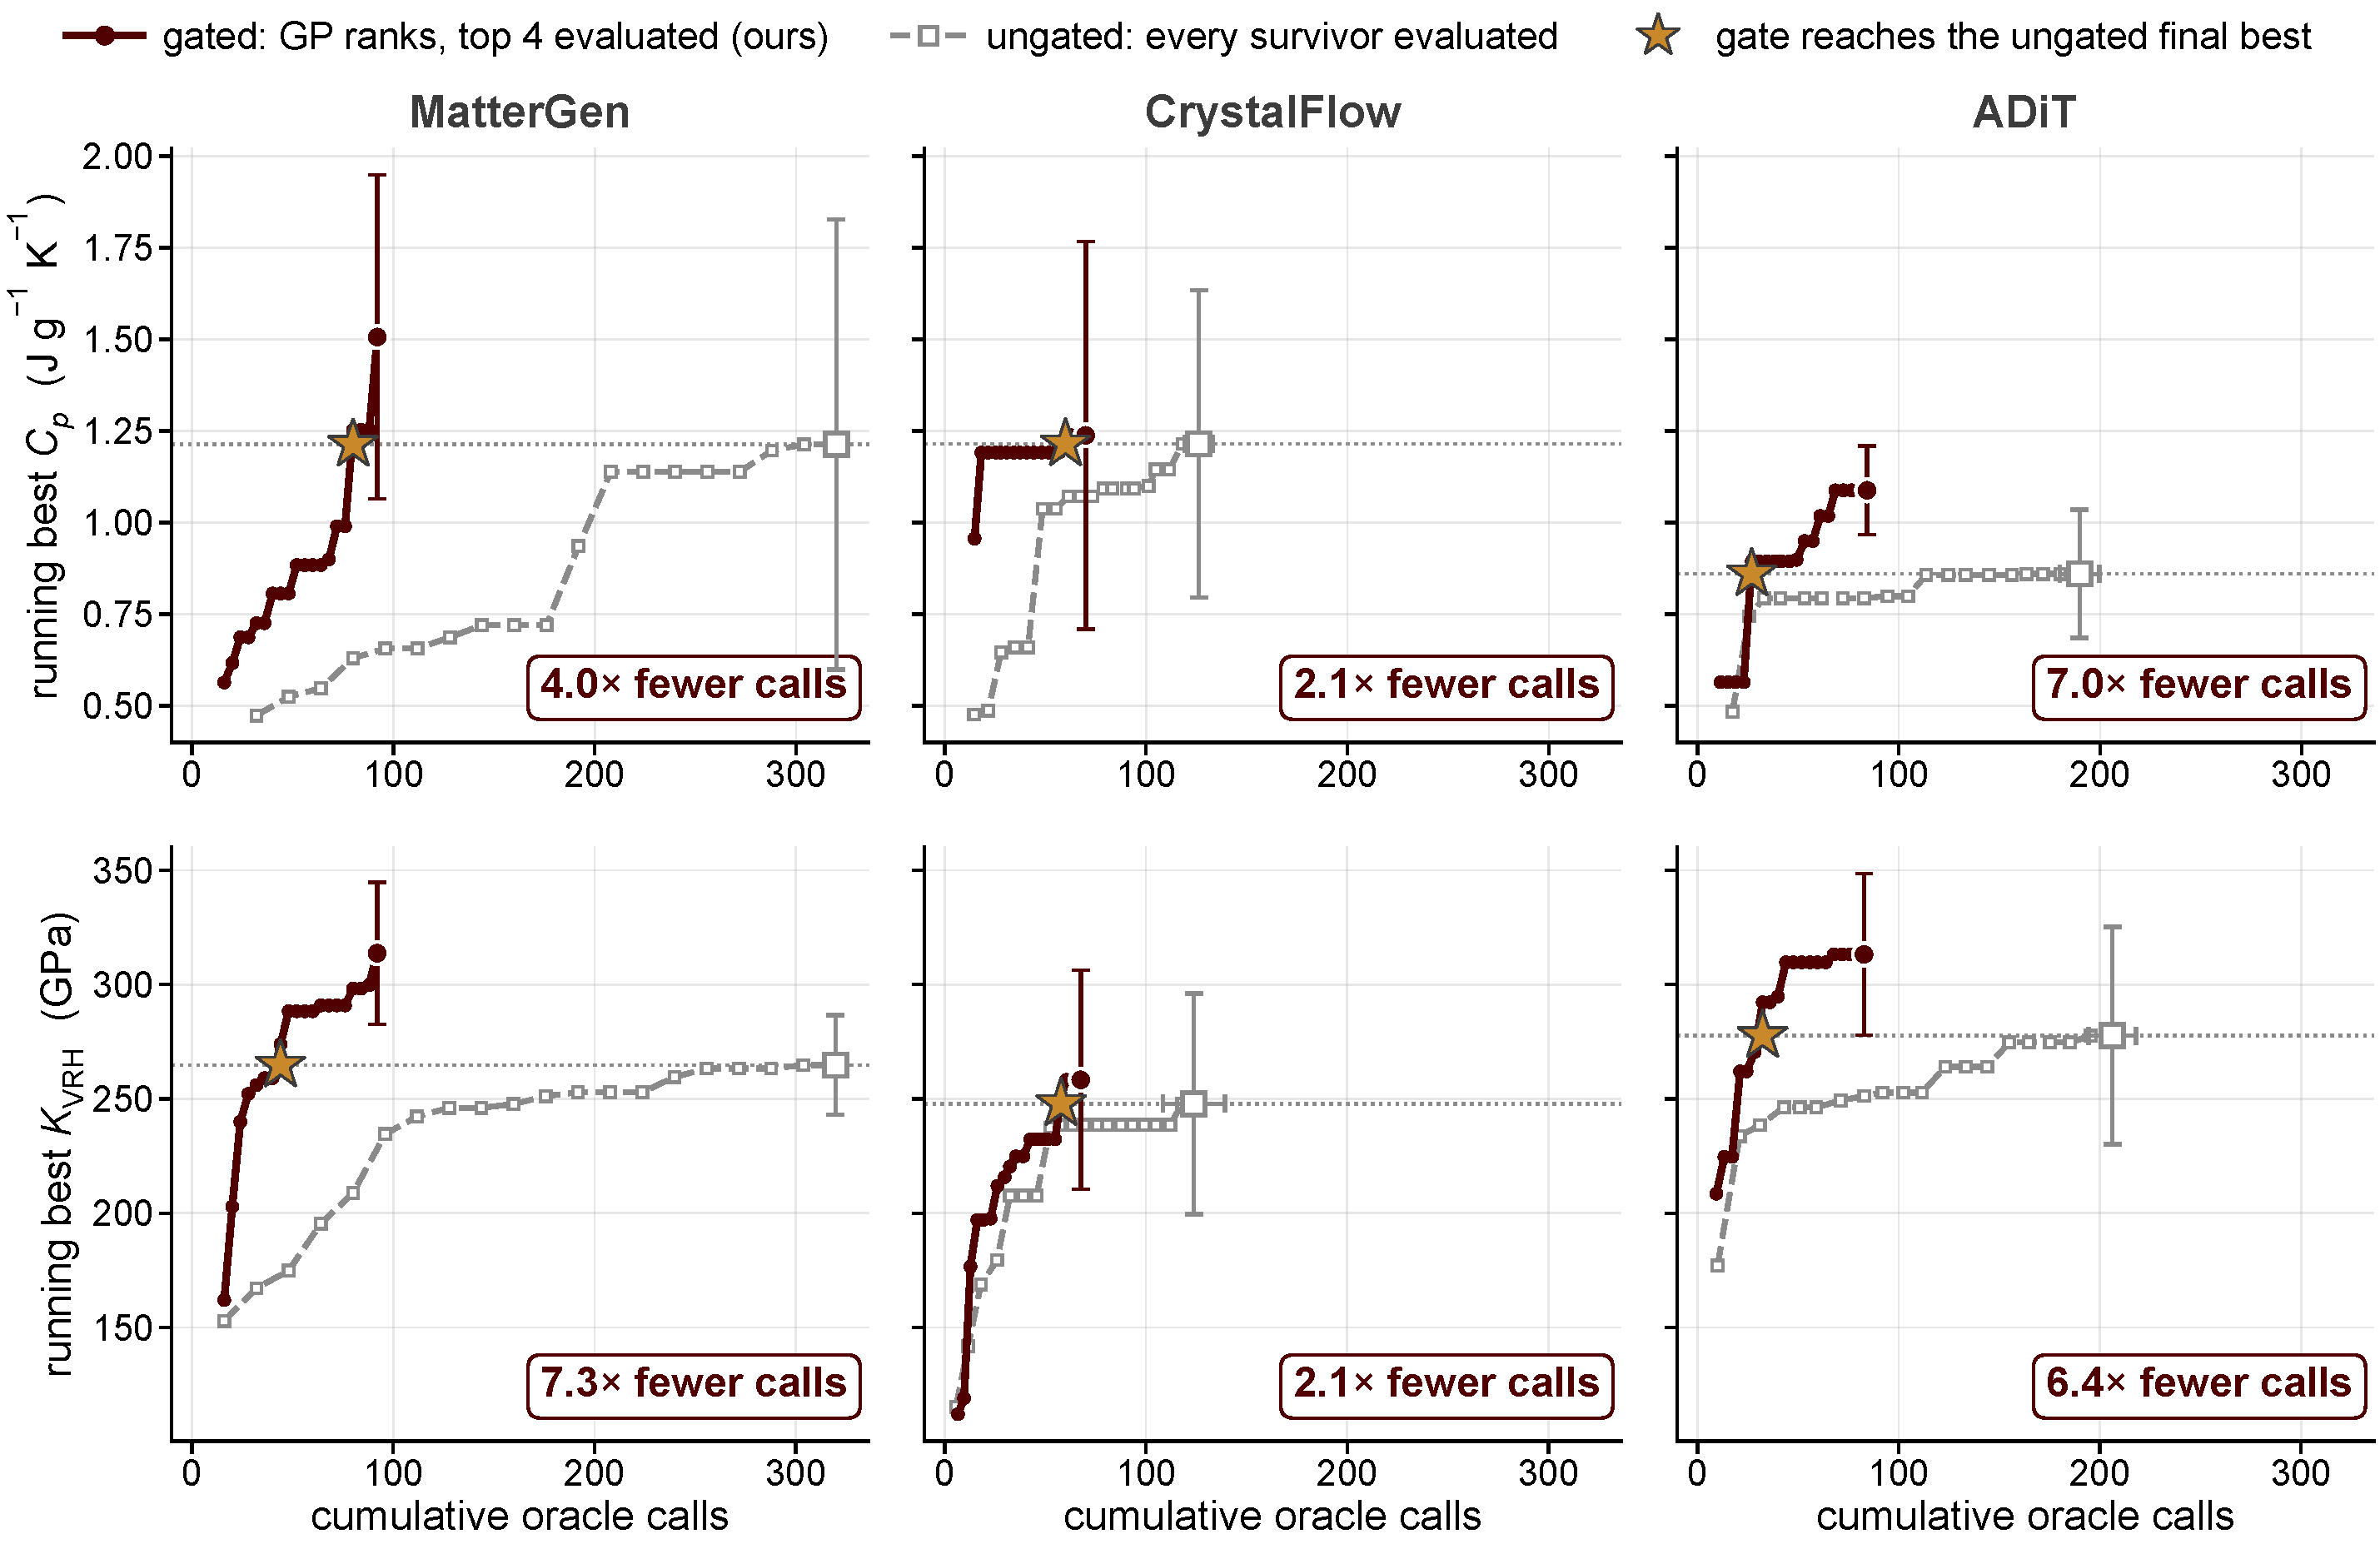
\includegraphics[width=\linewidth]{figs/fig_discovery.pdf}

\vspace{0.30cm}
\raggedright
Running best property against cumulative oracle calls: heat capacity
(top) and bulk modulus (bottom). Lines are seed means (five seeds; four
for gated ADiT heat capacity), bars one standard deviation. In every case
the gated policy reaches the ungated final best with 2.1 to 7.3
times~fewer~calls.
\end{posterbox}

\vfill

\begin{posterbox}[left=0.9cm,right=0.9cm]{\secno{5}Selection, Not Budget, Drives Discovery}
\centering
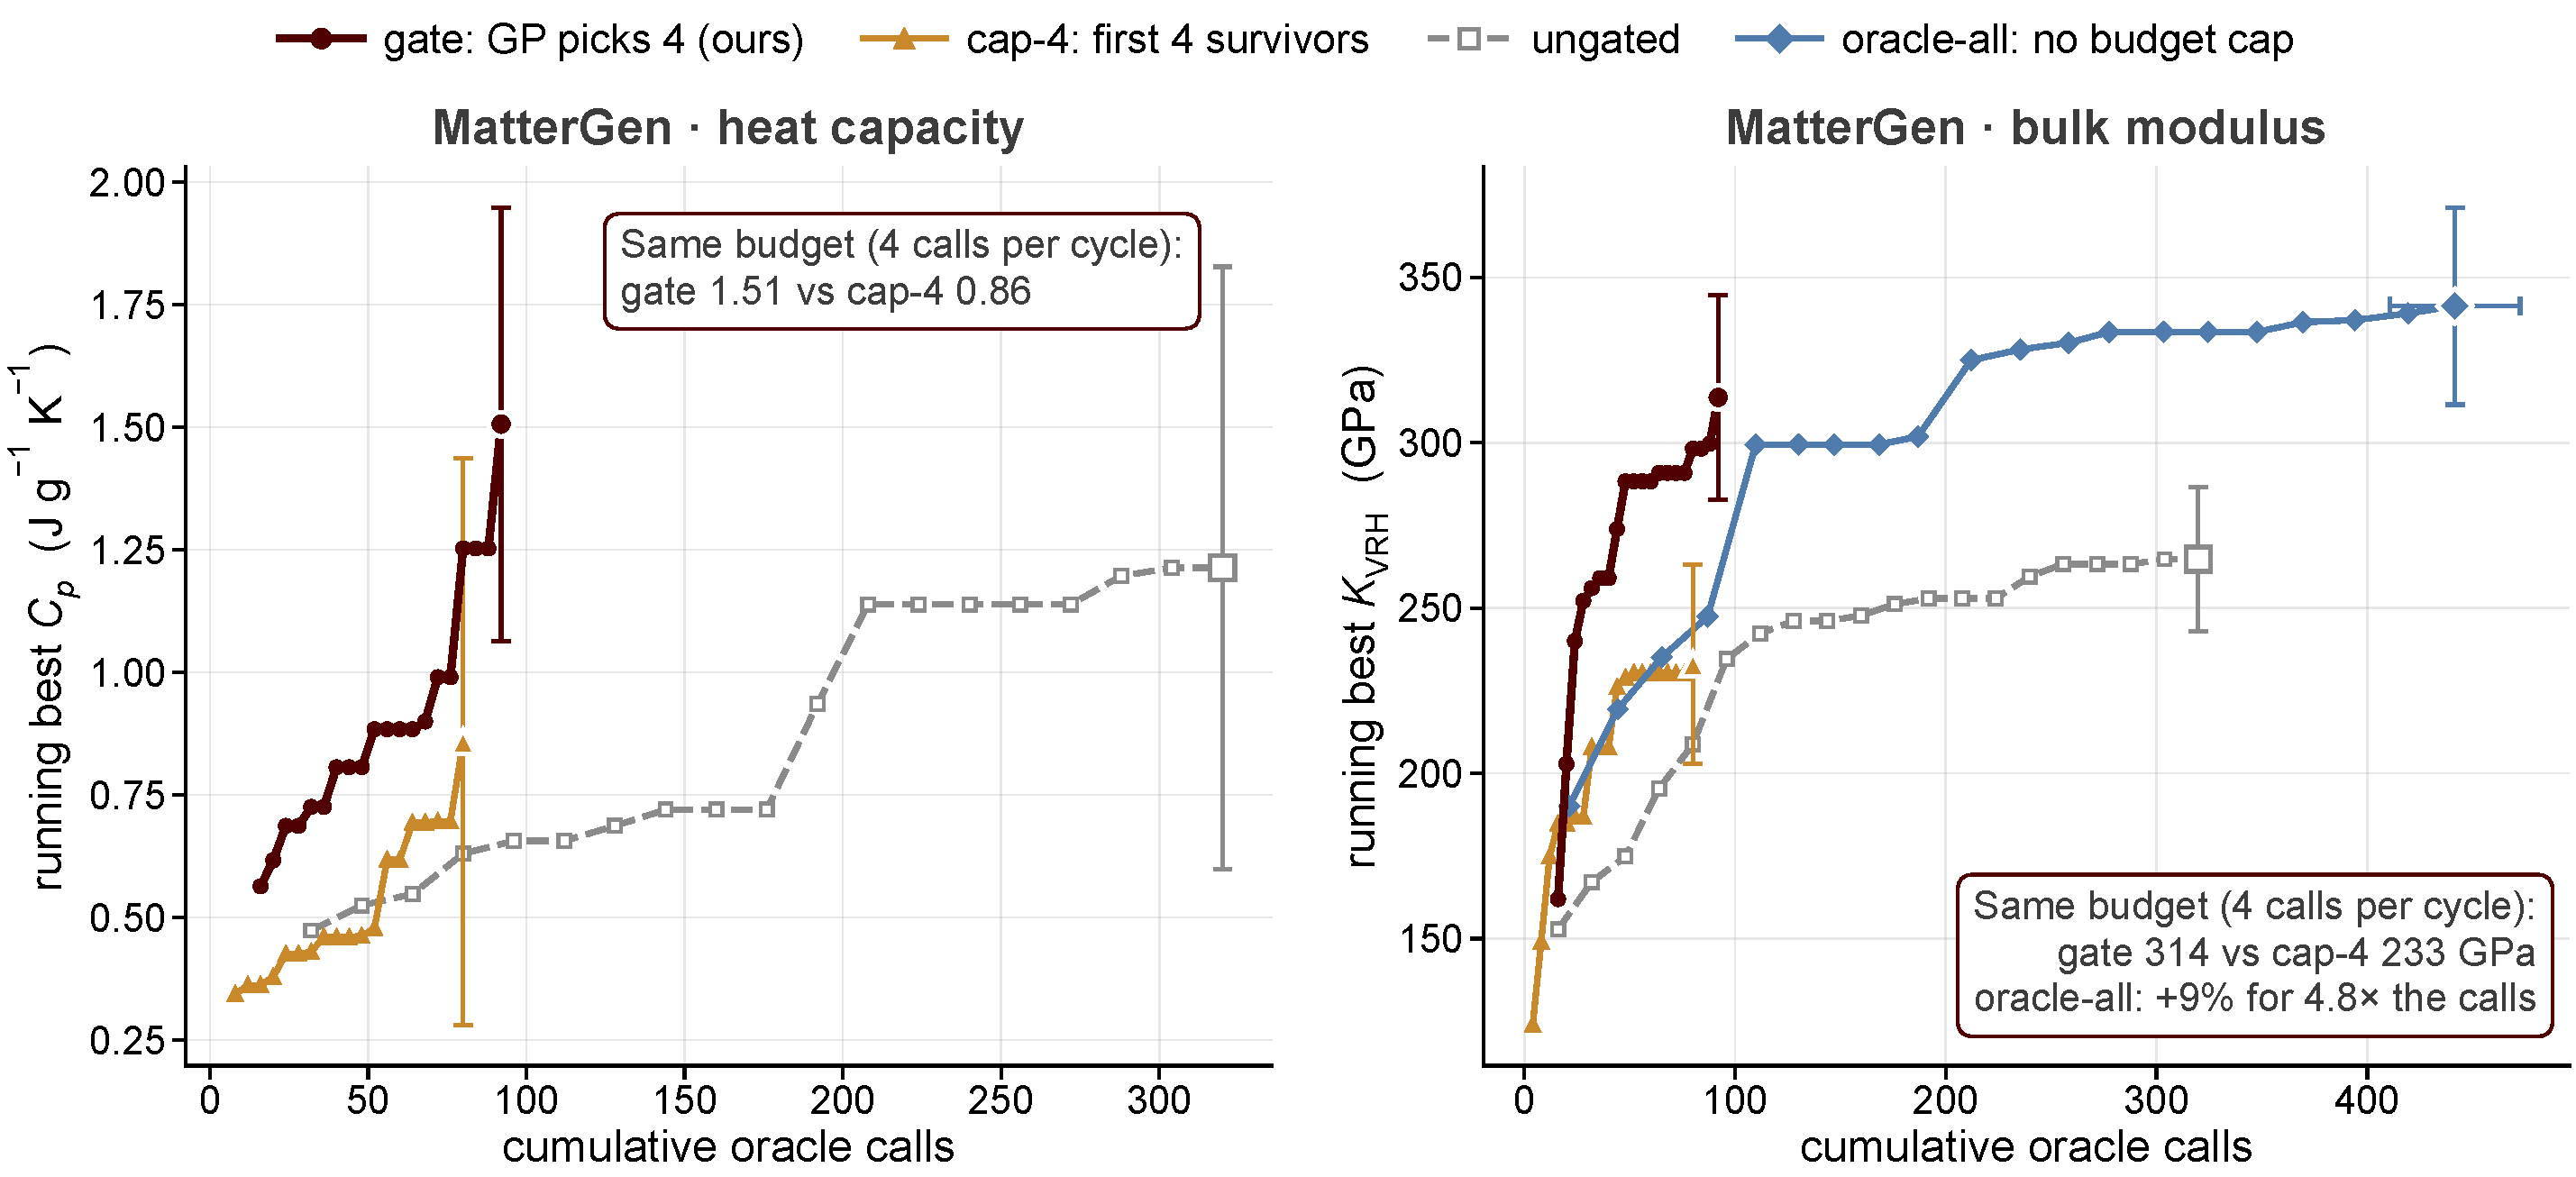
\includegraphics[width=\linewidth]{figs/fig_ablation.pdf}

\vspace{0.30cm}
\raggedright
MatterGen with the generation front end held fixed. Four arbitrary
survivors per cycle (cap-4) fall below ungated fine-tuning; four chosen
by the Gaussian process reach 314~$\pm$~31~GPa. Removing the budget cap
adds 9\% at 4.8 times the cost.
\end{posterbox}

\end{postercol}

%======================= COLUMN 3: validation and outcomes =======================
\begin{postercol}{\colw\textwidth}

\begin{posterbox}{\secno{6}Checked Against DFT}
\centering
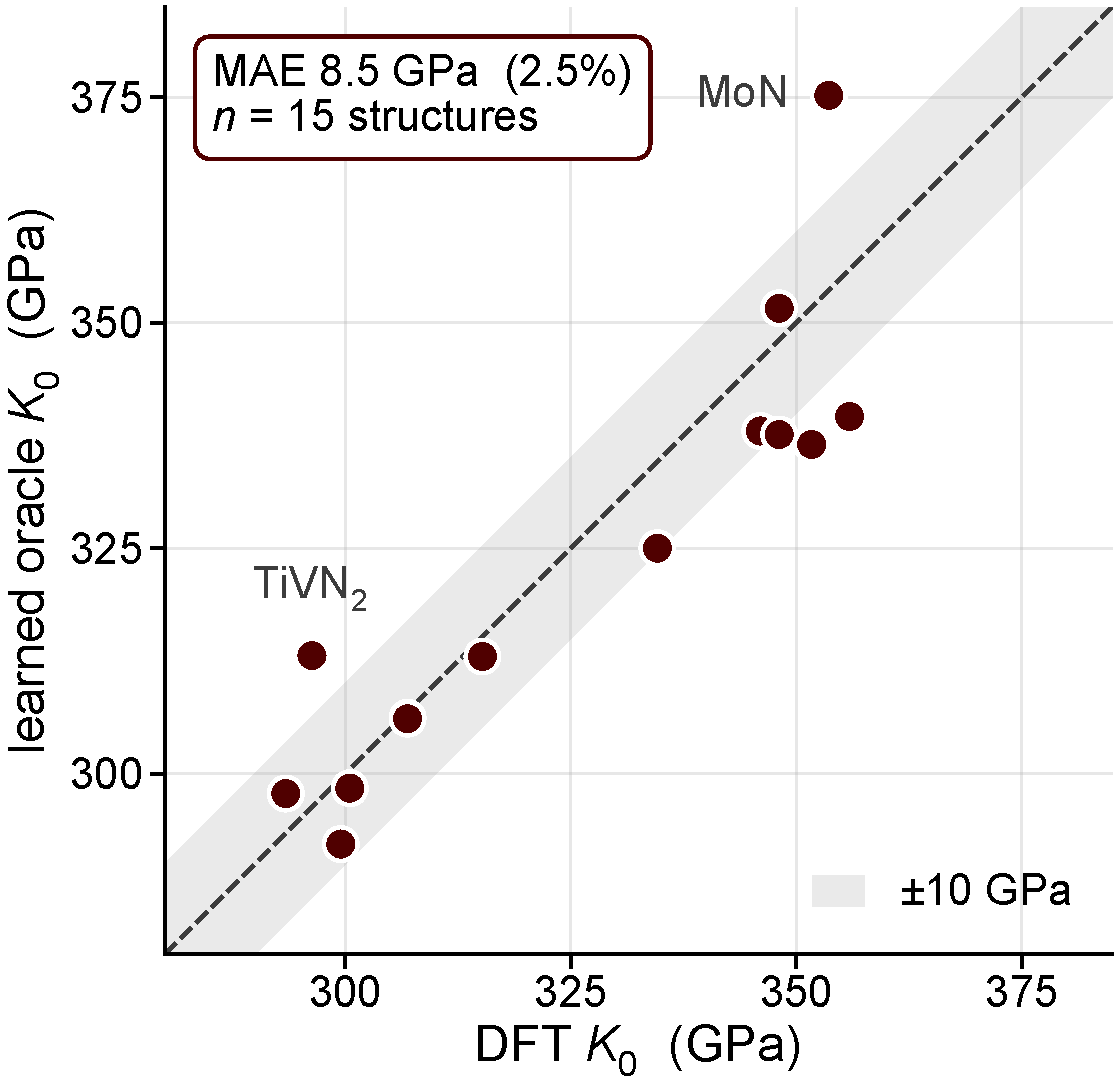
\includegraphics[width=0.87\linewidth]{figs/fig_dft_oracle.pdf}
\figcaptionc{\textbf{Oracle.} On the 15 top bulk-modulus structures the
learned oracle agrees with DFT to 2.5\%.}

\vspace{0.50cm}
\centering
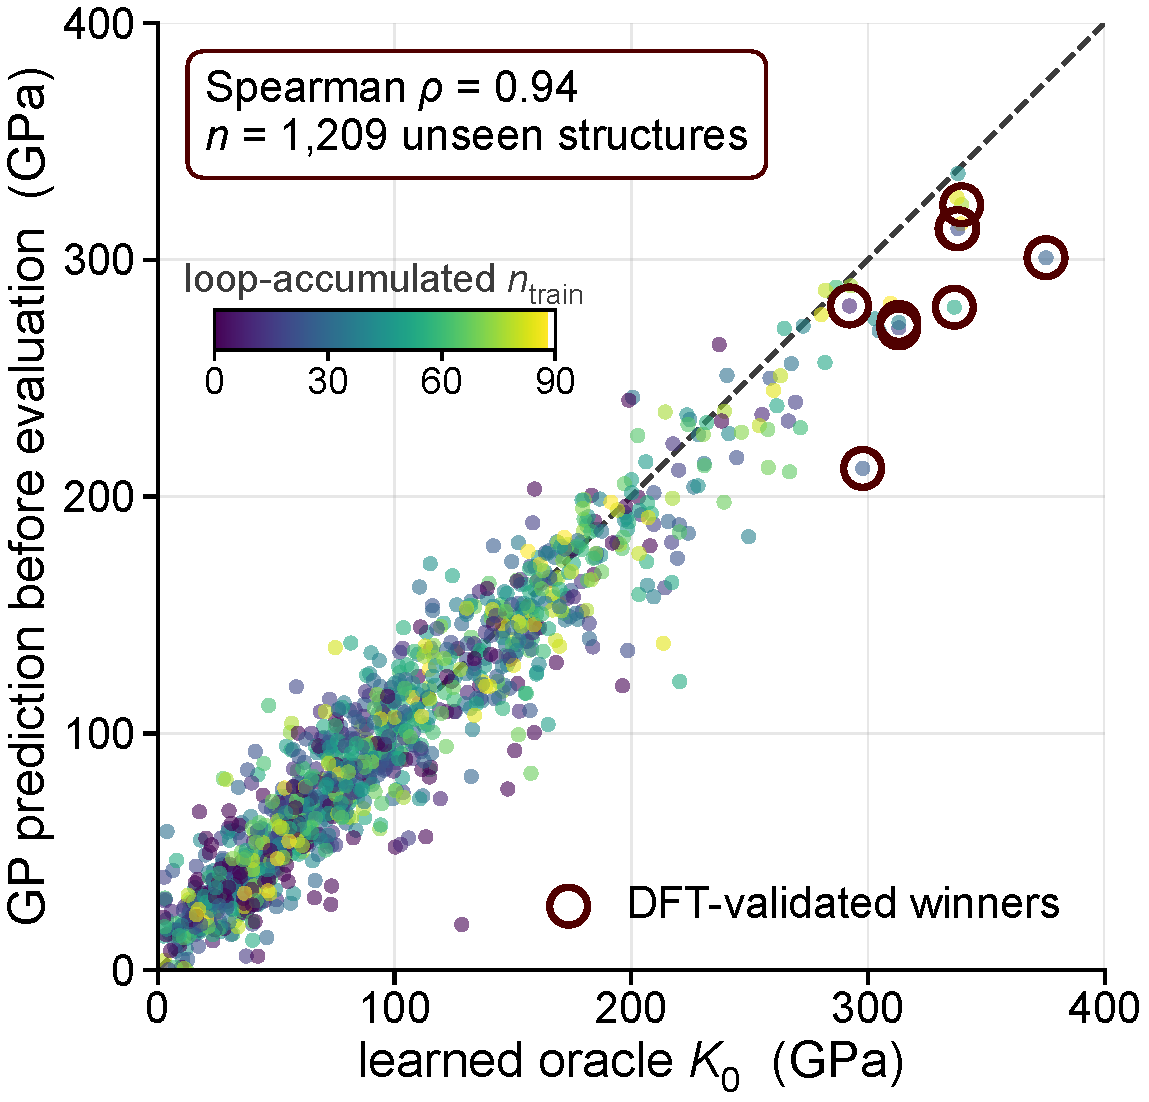
\includegraphics[width=0.87\linewidth]{figs/fig_dft_surrogate.pdf}
\figcaptionc{\textbf{Surrogate.} Trained only on earlier cycles (colour:
training points gathered by the loop), the Gaussian process orders new
structures at $\rho$~=~0.94 but underpredicts the hardest extremes: a
ranker, not~a~regressor.}

\vspace{0.35cm}
\raggedright
Limits: the oracle is a learned potential, and DFT validation covers
bulk modulus only.
\end{posterbox}

\vfill

\begin{posterbox}{\secno{7}Structures Found}
\centering
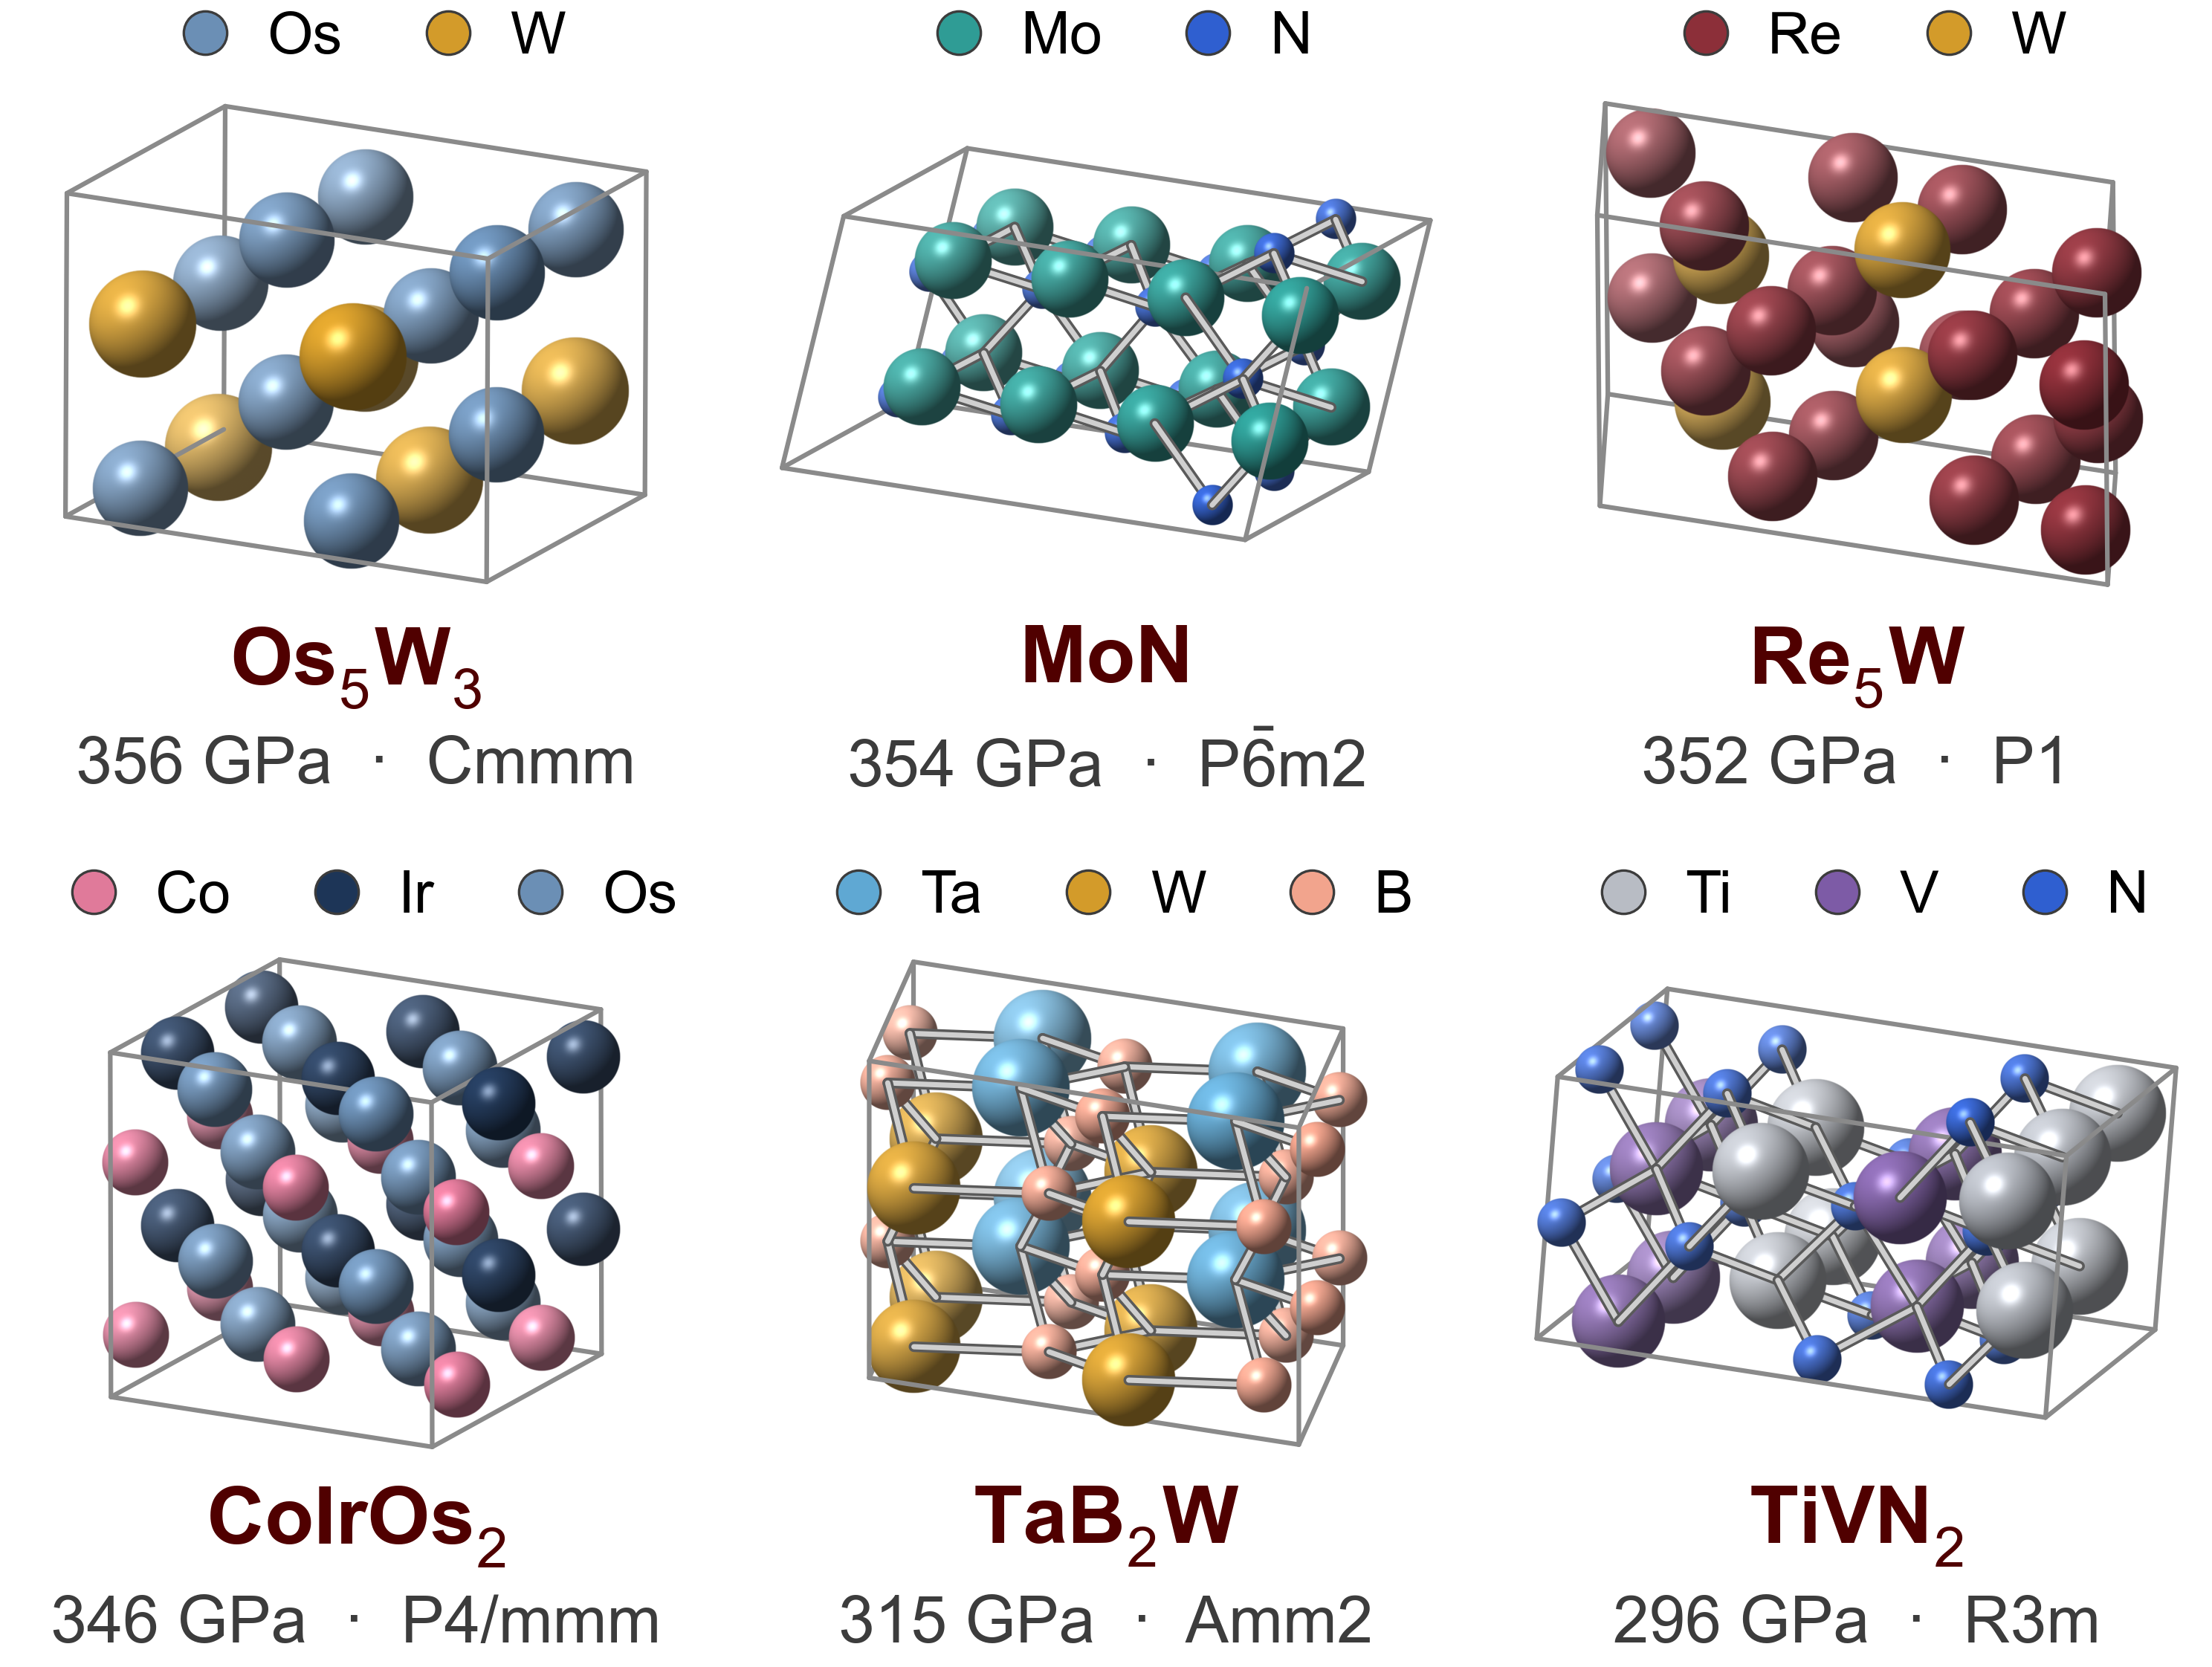
\includegraphics[width=\linewidth]{figs/fig_structures.png}
\figcaptionc{DFT-validated structures from gated runs of all three
priors (DFT bulk modulus, space group). None of the 177 top structures
matches the warm-start pool.}
\end{posterbox}

\end{postercol}
\end{columns}

\posterfooterrule
\gatefooter
  {Chen \textit{et al.}, MatInvent, arXiv:2511.03112 (2025).\quad
   Zeni \textit{et al.}, MatterGen, \textit{Nature} (2025).\\
   Luo \textit{et al.}, CrystalFlow, \textit{Nat.\ Commun.} (2025).\quad
   Joshi \textit{et al.}, ADiT, arXiv:2503.03965 (2025).\\
   Neumann \textit{et al.}, Orb, arXiv:2410.22570 (2024).\quad
   Fu \textit{et al.}, eSEN, arXiv:2502.12147 (2025).}
  {Supported by the Texas A\&M University System National Laboratories
   Office and Los Alamos National Laboratory (Joint Research Collaboration
   Program) and the U.S.\ DOE ARPA-E CHADWICK program (DE-AR0001988).
   Computing: Texas A\&M HPRC and NSF ACCESS allocation MAT250131 (ACES).}

\end{frame}
\end{document}
